\documentclass[UTF8]{ctexart}
\usepackage{graphicx}
\usepackage{float}
\usepackage{geometry}
\usepackage{fancyhdr}
\usepackage{lastpage}
\usepackage{enumerate}
\usepackage{multirow}
\usepackage{booktabs}
\usepackage{geometry}
\usepackage{amsmath}
\usepackage{mathrsfs}
\usepackage[linesnumbered,boxed,ruled,commentsnumbered]{algorithm2e}
\geometry{left=2.54cm,right=2.54cm,top=3.18cm,bottom=3.18cm}%页边距
\pagestyle{fancy}
\lhead{
\includegraphics[scale=1]{sjtu-logo-red.pdf}}  
\rhead{多种方法实现的三维脑肿瘤分割} 
\cfoot{第 \thepage\ 页\ 共 \pageref{LastPage} 页} 

\begin{document}

\begin{titlepage}
    \begin{center}
        
\includegraphics[width=0.8\textwidth]{sjtu-name-blue.pdf}\\[1cm]
        \textsc{\Huge \bfseries 课程报告}\\[1.5cm]
        
\includegraphics[width=0.3\textwidth]{sjtu-badge-blue.pdf}\\[0.5cm]    

        \Huge \bfseries{多种方法实现的三维脑肿瘤分割项目报告}\\[1cm]
        \Large \bfseries{518021910971 裴奕博}\\
        \Large \bfseries{518021910795 丁一}\\
        \Large \bfseries{518082910006 陈波}\\
        \Large \bfseries{518021910637 栗行健}
    \end{center}
\end{titlepage}
\tableofcontents
%正文

\newpage
\section{项目简介}
\subsection{项目概述}
本项目采用了阈值分割,区域增长等多种分割算法,结合形态学处理等辅助增强手段,对给定的脑肿瘤进行了分割,并取得了不错的效果。整个项目均采用自己实现的Python算法,项目的总流程如下:
\begin{figure}[H]
    \centering  %图片全局居中
    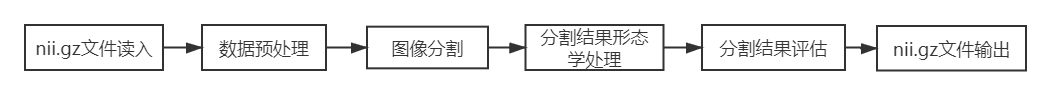
\includegraphics[width=\textwidth]{figure/workflow.png}
    \caption{总工作流程图}
\end{figure}
其中:
% TODO
\begin{itemize}
    \item nii.gz文件的输入输出均由SimpleITK包完成
    \item 数据预处理部分的算法包括 % TODO
    \item 图像分割算法包括:去除背景的三维Otsu算法,传统的三维区域增长算法,改进后的三维区域增长算法。
    \item 分割结果的形态学后处理方法包括:开运算和闭运算操作。
\end{itemize}

\subsection{采用数据}
我们组的编号为04,采用的数据集是Dataset\_Group/04文件夹下的三个待分割样本,编号分别为$BRAT\_008,BRAT\_033,BRAT\_259$。


\subsection{各文件(夹)功能}
\begin{itemize}
    \item README.md文件:说明了本项目的主要信息和使用方法。
    \item requirements.txt文件:说明了本项目所需环境中的依赖包。
    \item Dataset\_Group文件夹:存放待分割样本和标签。
    \item train\_data文件夹:存放经切片之后的二维图像,可供深度学习使用。
    \item output文件夹:存放经过算法之后输出的文件,文件夹下共由5个子文件夹,对应5种分割和结果后处理的方法。
    \item run.bat文件:命令行运行脚本,用户若需要再不同的分割方式下进行切换,可以直接在该文件中修改参数实现。
    \item main.py文件:整个项目的主函数,包含了从数据读入,调用算法和结果评估,输出结果的全过程。
    \item iotest.py/sitk\_test.py/iotest.nii.gz文件:项目实现过程中的调试文件和调试输出,用户使用时不要运行。
    \item otsu.py文件:实现了三维的Otsu阈值分割函数。
    \item region\_growing.py文件:实现了三维的区域增长分割函数。
    \item validation.py文件:实现了混淆矩阵(confusion matrix)和所有评价指标的求取。
    \item visualize.py文件:输出分割的可视化结果。
    \item config.py文件:存放算法过程中所需的常量。
    \item utils.py文件:实现算法过程中其余所有需要用到的辅助函数(如输入输出、可视化、形态学算法等)
    \item result.json文件:存放分割算法的评价指标原始数据。
    \item result\_to\_csv.py文件:将json中的原始数据读出后转换并整理为csv格式。
    \item result.csv文件:存放本项目各方法的最终对比结果。
\end{itemize}

\subsection{使用说明}
见README.md文件中run部分。

\section{实现思路与方法}
\subsection{基于多阈值Otsu的图像分割}
从数据集和标签的对比中我们可以看到,脑肿瘤对应的区域基本为原图的高亮区,与周围组织灰度相差较大,因此最简单直接的思路就是考虑直接通过阈值处理进行分割,由于要自动选择阈值,因此我们采用了Otsu算法,并将其扩展至三维。

\subsubsection{传统的多阈值Otsu方法}
传统二阈值Otsu算法的基本假设如下:假定图像包含几类像素,直方图为多峰直方图,然后计算使得多类像素能分开的最佳阈值(类内方差),或等价的间类间方差最大。

写成伪代码将思路表示如下:

\begin{algorithm}[H]
    \caption{Traditional Otsu}\label{algorithm}
    \KwIn{img: 3d-array of size $w\times h\times q$}
    \KwOut{result,t1,t2}
        Initialize t1,t2,result\;
        $m_g$=mean(img)\;
        \For {t1 = 0 to GRAY\_MAX}{
            \For{t2 = 1 GRAY\_MAX-1}{
                m1=mean(img[img<t1])\;
                p1=count(img[img<t1])\;
                m2=mean(img[img>t1 and img<t2])\;
                p2=count(img[img>t1 and img<t2])\;
                m3=mean(img[img>t2])\;
                p3=count(img[img>t2])\;
                var[t1][t2]=$p1*(m1-m_g)^2+p2*(m2-m_g)^2+p3*(m3-m_g)^2$\;
            }
        }
        t1,t2=argmax(var)\;
        result=img[img>t2]\;
        \Return{result,t1,t2}
        
\end{algorithm}

	t1,t2即为所求。Otsu方法可以形象地理解为:求取直方图多个峰值之间的低谷值t1,t2。
\subsubsection{改进后的Otsu方法}
使用传统的Otsu算法之后,发现对部分样本效果不佳,原因是在整个三维图像中,背景像素(即灰度值接近0的像素)过多,也输出了很多噪点,导致最后输出的结果不佳。因此我们对传统的Otsu算法进行了一下几点改进:
\subsubsection*{阈值与背景处理}
经过改进,我们将所有灰度值小于某阈值t(实际取值为10)的像素点忽略,不计入均值和方差的计算中。这一改进既提升了算法的速度,又避免了大面积背景的影响。


\subsubsection*{添加形态学后处理}
仅用上述改进的otsu代码分割肿瘤时出现了两处问题:
\begin{itemize}
    \item 肿瘤外部有独立小分区(来源于图像的独立高亮噪点)。
    \item 肿瘤内部出现未闭合区域(来源于原图像肿瘤区域中的暗区)。
\end{itemize}

为了有效避免这两种情况的出现,我们对解雇采取了形态学操作的后处理方法,采用了先闭运算后开运算的方法。闭运算→开运算:闭运算(先膨胀再腐蚀)可以填平小孔,弥补小裂缝,并保持总的位置和形状不变;开运算(先腐蚀再膨胀)可以去除孤立小点,毛刺和小桥,总的位置形状不变。故结合闭运算和开运算进行预处理,有效避免了直接otsu处理所产生的两处问题,提高了分割的有效性。

\subsubsection*{同直接遍历对比}

直接遍历图像得到能够用于分割图像的阈值点,一般用手动选择的方式确定分割阈值,从算法复杂度看,直接遍历和otsu是相同的,但是由于otsu可以自动选择合适的阈值且有合理的数学依据,相比直接遍历的人工选择有着巨大的优势。

\subsubsection*{改进后的算法}
经过以上几点改进,我们的算法思路可以表示如下:

\begin{algorithm}[H]
    \caption{Our new Otsu}\label{algorithm}
    \KwIn{img: 3d-array of size $w\times h\times q$, t:int}
    \KwOut{result,t1,t2}
        Initialize t1,t2,result\;
        $m_g$=mean(img)\;
        \For {t1 = t+1 to GRAY\_MAX}{
            \For{t2 = t+2 GRAY\_MAX-1}{
                m1=mean(img[img<t1 and img>t])\;
                p1=count(img[img<t1 and img>t])\;
                m2=mean(img[img>t1 and img<t2])\;
                p2=count(img[img>t1 and img<t2])\;
                m3=mean(img[img>t2])\;
                p3=count(img[img>t2])\;
                var[t1][t2]=$p1*(m1-m_g)^2+p2*(m2-m_g)^2+p3*(m3-m_g)^2$\;
            }
        }
        t1,t2=argmax(var)\;
        result=img[img>t2]\;
        result=opening(closing(result))\;
        \Return{result}
        
        
\end{algorithm}

\subsubsection{otsu算法总结}

	我们使用的三维otsu算法从最终结果上看是符合要求的,最初我们有想通过分割成155张二维图像分别进行otsu处理(其结果与三维处理相同),但是这是间接进行分割,在实际应用中可能会碰到繁冗步骤与分割的不确定性,故改写otsu算法可以对三维图像进行直接处理,由于去除了背景,大大降低了运算时间并提高了阈值的准确度。为了更好地分割图像,我们去除了背景,添加了闭运算与开运算进行后处理,去除了孤立区域(亮点与暗点)。整体而言,otsu算法在此类有着较为明显区间阈值差异图像中有很好的体现,但是缺陷比较明显,在肿瘤区域高亮时容易分割,区域高亮但是有明显灰度值差异如800和1000左右的差异,会导致阈值的选取出现异常,出现较大的暗区或者分割部分变小。正因如此,我们考虑到了区域增长的办法进行图像分割。




\subsection{基于区域增长的图像分割}
\subsubsection{传统的区域增长方法}
区域生长是根据事先定义的准则将像素或者子区域聚合成更大区域的过程。其基本思想是从一组生长点开始(生长点可以是单个像素,也可以是某个小区域),将与该生长点性质相似的相邻像素或者区域与生长点合并,形成新的生长点,重复此过程直到不能生长为止。生长点和相似区域的相似性判断依据可以是灰度值、纹理、颜色等图像信息。所以区域生长算法关键有三个:
\begin{itemize}
    \item 选择合适的生长点
	\item 确定相似性准则即生长准则
	\item 确定生长停止条件
\end{itemize}
根据输入图像,我们同样将其扩展至三维,传统的区域增长方法可以表示如下:

\begin{algorithm}[H]
	\caption{Traditional region growing}\label{algorithm}
    \KwIn{img: 3d-array of size $w\times h\times q$,seed: list of len=3, radius:int, t:int}
    \KwOut{ifsearch}	
    Initialize ifsearch,head,tail,region\_queue\;
    \While{head<tail}{
        center=region\_queue.pop()\;
        head++\;
        \ForAll{point in distance(point,center)<radius}{
            \If{abs(img[point]-img[center]<t)}{
                ifsearch[point]= 1\;
                region\_queue.push(point)\;
                tail++\;
            }
        }
    } 
    
    \Return{ifsearch}
\end{algorithm}

\subsubsection{改进后的区域增长方法}
在区域增长算法的使用过程中,我们发现了各种问题,比如在有些样本中,区域很难向外生长,而在另一部分样本中,增长的区域与正常脑组织混杂难以收敛,区域出现空洞等各种问题,因此我们对传统的区域增长方法也加以了几点小小的改进。

    \subsubsection*{高亮区域分割的去绝对值处理}

    区域增长的传统判定标准是abs(img[point]-img[center]<t),我们按照这个思路进行分割时会出现区域难以增长的现象,这是因为肿瘤高亮部分会有一部分灰度值过大,在区域增长中被排除在外(在样本中出现了只增长几十个点的情况)。故改进后的算法去掉了abs,即将所有大于邻域中心灰度值的点都采纳,这样肿瘤中高亮部分能够全部被囊括,能够提高统计学的有效性判断。
    \subsubsection*{闭运算后处理}

    由于肿瘤区域存在部分暗区或者孤立暗点,故利用闭运算的方式来填充孔洞,弥补缝隙,使得增长区域更加完整。但由于在区域增长中,增长区域连续的程度显然比用阈值处理的结果高得多,因此这一后处理的效果在不同样本上体现的效果也有较大差异。

    \subsubsection*{强制终止迭代}

    在代码调试阶段,由于阈值和种子点选取不同,有时会导致区域增长出现越界现象,即将整个脑区增长完,同肿瘤区的几万个点相比,脑区总点数超过百万,故我们设定了强制终止点,当生长开始后所判断符合要求的点数超过终止数时停止生长。这样做可以在一定程度上能够限定区域增长总是在肿瘤区附近,不会出现增长区域扩散至整个脑区的现象。这一改进对于肿瘤在某个方向上与脑区界限比较模糊的状况有着良好的效果。

    \subsubsection*{改进后的算法}
    
    \begin{algorithm}[H]
        \caption{Our new region growing}\label{algorithm}
        \KwIn{img: 3d-array of size $w\times h\times q$,seed: list of len=3, radius:int, t:int,tailmax:int}
        \KwOut{ifsearch}	
        Initialize ifsearch,head,tail,region\_queue\;
        \While{head<tail}{
            \If{tail>tailmax}{
                break\;
            }
            center=region\_queue.pop()\;
            head++\;
            \ForAll{point in distance(point,center)<radius}{
                \If{img[point]-img[center]>t}{
                    ifsearch[point]= 1\;
                    region\_queue.push(point)\;
                    tail++\;
                }
            }
        }
        \For{i =head to tail}{
            ifsearch[region\_queue[i]]=1
        }
        ifsearch=closing(ifsearch)
        \Return{ifsearch}
    \end{algorithm}

    

    \subsubsection{区域增长算法总结}
    在我们选用的样本中,区域增长和ostu算法各有优劣,从算法原理上看,区域增长更适合作为分割肿瘤的处理手段,不过由于医学图像肿瘤区的高亮特性,利用otsu算法也能够得到比较好的结果。区域增长由于可以不断调整参数,能够人为的提高分割的准确性,在医学分割领域有更好的前景。

	区域增长在设计好各项参数后,能够得到比其余分割算法更好的结果。在医学图像中,肿瘤一般具有高亮且边缘明显的特征,利用区域增长处理图象时,要么得到肿瘤区域,要么得到非肿瘤区域,这两种结果都可以有效分割出期望结果。但是由于区域增长原理,有时会出现过度增长甚至全局增长的结果,此时需要进行图像预处理或人工参数设定与代码优化。总体而言,区域增长在医学领域有着较好的应用前景。



\section{项目评价}
\subsection{评价指标介绍}
	
    基于我们预测出来的肿瘤图像与标准标注的肿瘤图像进行比较,我们将每个像素看作一个样本,则每张图都可看作一个二分类模型的数据集。我们采用一系列二分类的评价指标进行对算法性能的分析,用以判断每张图中我们预测的肿瘤与金标准的贴合程度,这些指标主要由TP、FP、TN、FN计算得到。
    \begin{itemize}
        \item TP(True Positive)表示真阳性,表示预测与标准都为真,在这里统计为预测和标准的像素值都为1的像素个数;
        \item FP(False Positive)表示假阳性,表示标准为假,但预测判断为真,也被称为I类错误,在这里统计为预测的像素值为1,标准的像素值为0的像素个数;
        \item TN(True Negative)表示真阴性,表示预测和标准都为假,在这里统计为预测和标准的像素值都为0的像素个数;
        \item FN(False Nagetive)表示假阴性,表示标准为真,但预测判断为假,也被称为II类错误,在这里统计为预测的像素值为0,标准的像素值为1的像素个数。
    \end{itemize}
	
	
	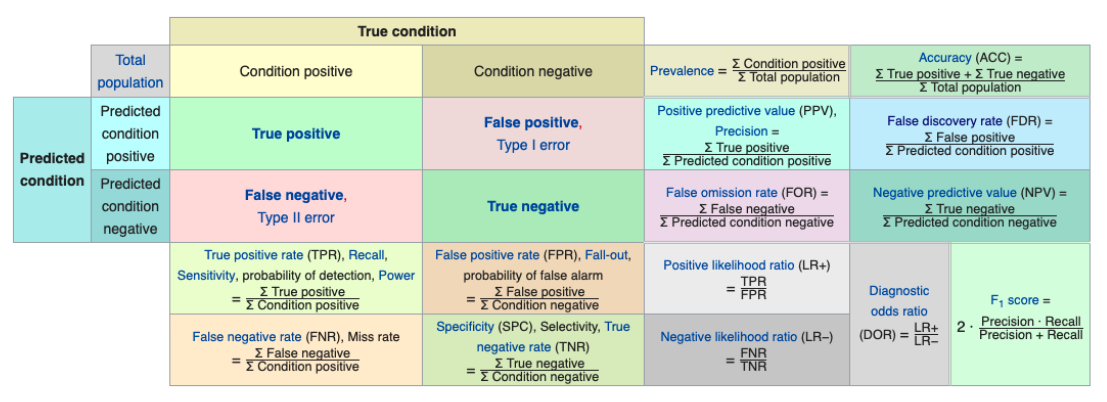
\includegraphics[width=0.8\textwidth]{figure/valid.png}
	
	下面,我们定义敏感度sensitivity、特异性specificity、准确率precision、精确度accuracy、交并比IoU和dice相似系数,由下列公式给出:
    \begin{equation}
        \begin{aligned}
            &sensitivity = \frac { TP } { TP + FN } \\
            &specificity = \frac { TN } { FP + TN }\\
            &precision = \frac { TN } { TP + FP } \\
            &accuracy = \frac { TP + TN } { TP + TN + FP + FN }\\
            &IoU = \frac { TP } { TP + TN + FP}\\
            &dice = \frac { 2 \times TP} { 2 \times TP + TN +FP} 
        \end{aligned}
    \end{equation}
	
	其中敏感度sensitivity可以通俗地理解为在金标准的阳性结果(肿瘤部分)中,预测算法能够判断出来多少。在信息工程的领域,敏感度sensitivity又被称为召回率recall。与其对应的是特异性specificity,指的是在金标准的阴性结果(非肿瘤部分)中,预测算法能够判断出来多少。
	
	敏感度sensitivity也可以与准确率precision作对照,准确率precision可以理解为预测的肿瘤部分有多少是对的。一般来说,算法的敏感度sensitivity与准确率precision也是相互拮抗的,要追求高的准确率势必要牺牲敏感度,反之,要追求高的敏感度势必要牺牲准确率。因此,在敏感度与准确率之间寻求一定的平衡,使它们都能达到较好的结果,是极为重要的,我们可以用另一个指标——精确度accuracy综合衡量敏感度sensitivity与准确率precision。精确度反映了在所有结果中,算法有多少是预测准确的。precision和sensitivity的降低,都会导致accuracy的降低,一般情况下其能较好地反映二分类算法的好坏。
	
	然而,我们的二分类模型其实是一类图像识别的模型。对于识别肿瘤这样远小于背景尺寸的算法,如果使用accuracy作为判定的最主要指标会造成对背景的识别(即TN的占比)占据很大的权重,这是我们不想要的。所以我们很自然地在accuracy的计算中将分子分母中的TN同时去掉,这样就得到了IoU。它在图像识别中还具有特殊的意义,指预测的图像与标准标注图像的交集与并集的比,能很好的反应检测目标的预测结果与标注结果的重叠程度,所以IoU能作为我们衡量算法性能的主要指标。
	
	另外,dice相似系数类似于IoU,不一样的地方在于IoU直接在accuracy中去掉了TN,而dice还将TP的权重变为原来的两倍,以平衡去掉的TN。dice相似系数也可以作为这类图像识别的主要性能指标。

	最后,我们加入了运算时间来衡量算法的运算效率。由于accuracy和specificty受背景的影响大,在实测中几乎都接近于$100\%$,所以没有很大的意义。最终我们选择敏感度sensitivity、准确率precision、交并比IoU、dice相似系数和运算时间time\_cost作为项目的评价指标。
\subsection{各方法效果比较}

\begin{figure}[H]
    \centering  %图片全局居中
    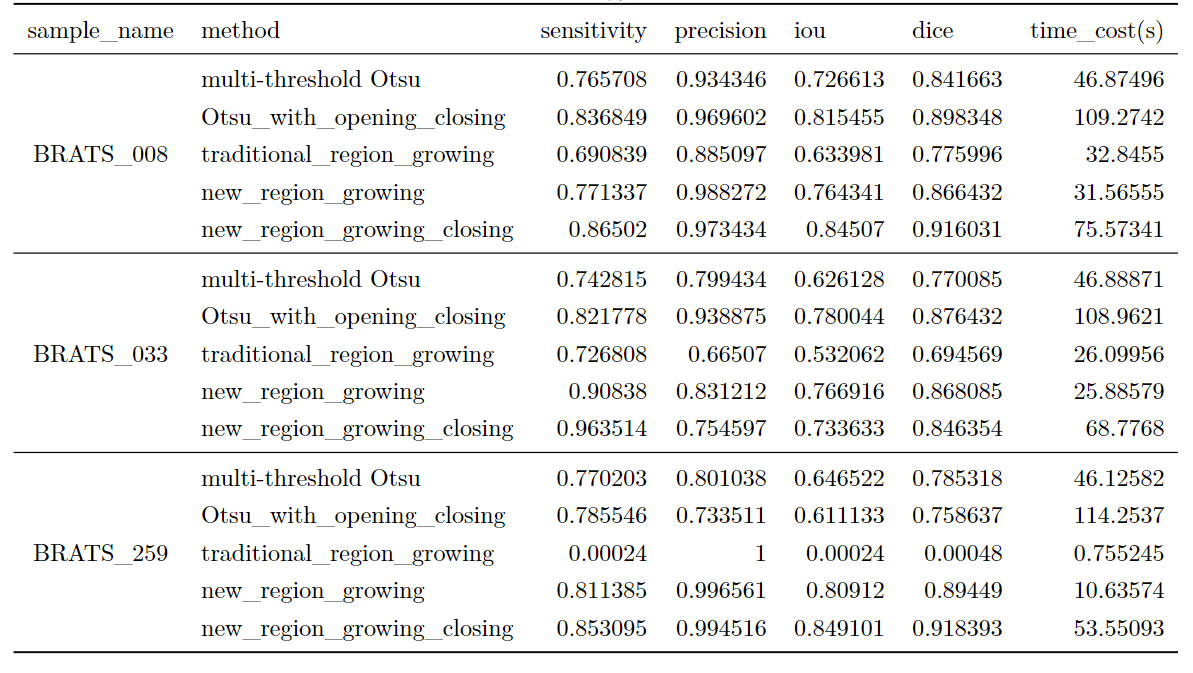
\includegraphics[width=0.9\textwidth]{figure/result_table.png}
    \label{tab:result}
    \caption{各方法评价指标比较表}
\end{figure}

  \begin{figure}[H]
    \centering  %图片全局居中
    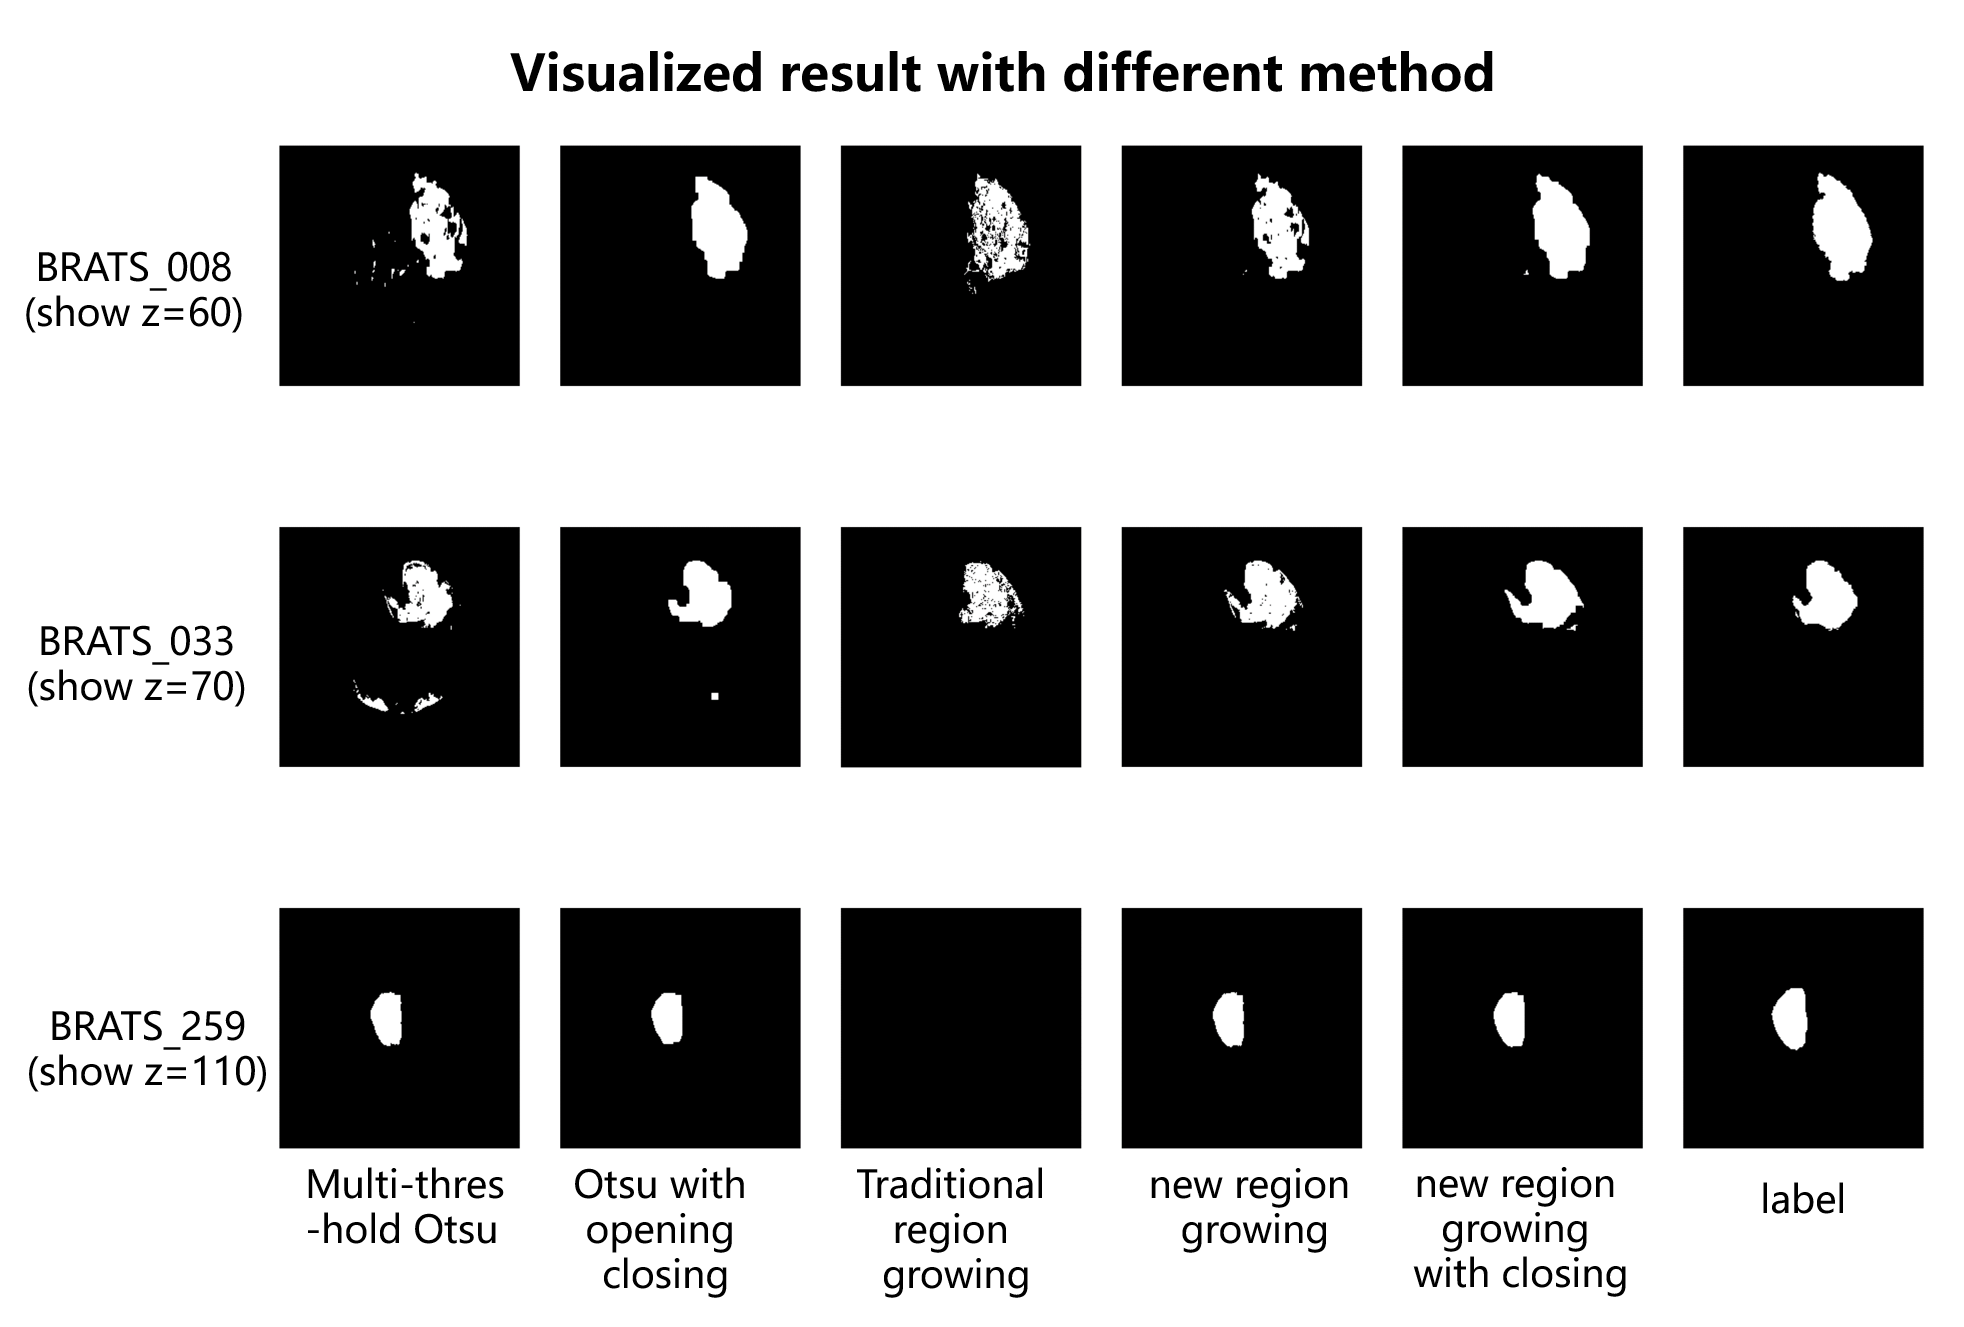
\includegraphics[width=0.8\textwidth]{figure/result.png}
    \caption{各方法可视化对比}
\end{figure}
		
	\subsubsection{otsu阈值算法的评价}
	在第二节中我们介绍了otsu二阈值算法实现对肿瘤的分割,下面我们先根据上述指标进行对otsu二阈值算法以及改进后的otsu二阈值算法的评价。我们选取我们组的三个样本得到的检测结果进行评价,具体结果如\ref{tab:result}所示:
	
	可以看到sensitivity和precision并未出现一个很高一个很低的情况,效果也较为不错。总体的IoU均达到了$60\%$以上,部分超过了$70\%$,还有一个甚至达到了$80\%$。通常IoU达到0.5以上算作击中,这样的结果可以初步认为otsu算法能较好地将肿瘤部分检测出来。
	
	对于前两个样本,改进后的otsu二阈值算法较改进之前有较明显的提升,而第三个样本中改进后的otsu算法的IoU不升反降。改进的方式主要是对原来的otsu算法进行了先闭后开的运算,其中闭运算是为了将肿瘤部分的一些孔洞填充,而开运算是为了消除除肿瘤外的一些噪点。根据图中的敏感度明显下降,我认为出现这种情况的主要原因是开操作将肿瘤的部分图像给腐蚀了。
	
	事实上,我们对一张图尝试过所有的阈值来验证otsu的二阈值算法是否取到了让IoU达到最佳的阈值,实验证明确实取到了最佳阈值。所以该类算法其实已经在阈值算法中做到了很好的结果,其不能再取得更好的结果主要是因为阈值算法总的来说还是有片面性的,它只利用了图像的像素大小信息,而并没有利用图像的位置信息。我们已经尽可能地利用开闭运算后处理加强对图像位置信息的利用,但提升并不是很大。
	
	\subsubsection{区域生长算法的评价}
	
	我们再根据之前所述指标进行对区域生长及其衍生算法的评价。同样,选取我们组的三个样本得到的检测结果进行评价,具体结果如\ref{tab:result}所示:
	
	对于第一个样本和第二个样本来说,sensitivity和precision达到了一个较好的平衡。使用未经过改进的区域生长算法,其IoU仅能达到$50\%$以上,而改进之后,其IoU均达到了$76\%$左右,经过闭操作后,第一个样本的IoU提高到了$84.5\%$,第二个样本的IoU不升反降,出现这种情况可能是因为闭操作使得区域生长超出范围的部分更大,而超过了空洞填充的有利影响,可以通过调小闭操作的结构元大小来使得结果变好。第三个样本中,使用未改进的区域生长算法后sensitivity变为0,是由于阈值在一开始就由于与周围像素的差值过大而终止了,所以并未生长出去;在改进的算法中,我们认为只要比当前像素亮的像素就一定是肿瘤,这样能够较好地避免由于差值过大而终止的情况。改进后的IoU达到了80以上,precision几乎接近于$100\%$,说明我们预测的图像几乎包含在标准标注的图像中,通过调整参数可能可以得到更高的IoU,但是为了使我们的区域生长方法具有一定的普适化能力,所以并未为了特定的样本去改变参数。而且,其经过闭运算的IoU也能达到$85\%$左右,我们认为已经达到了非常理想的结果。
	
	区域生长算法虽然取得了整体比otsu阈值算法更好的评价指标,但其有着比otsu阈值算法更大的局限性。首先,起始的种子需要自己寻找,即需要人工粗检测,属于非完全系统化的算法;其次,较难处理一些复杂情况,例如使用平凡的区域生长算法甚至在第三个样本最开始的生长阶段就被中断。另外,闭运算在区域生长中并没有取得明显的成效,部分图像的IoU上升而部分图像则不升反降,在未知标准标注的情况下,很难直接判断是否应该使用闭操作。

    \subsubsection{项目创新点}
    \begin{itemize}
        \item 在otsu阈值算法中,不考虑小于一定像素值的点,以排除周围较大块的黑色背景对阈值计算的影响,使得计算的阈值结果较为准确。
        \item 在区域生长算法中,认为较当前像素更亮的周围像素都将其认为是肿瘤部分,这是基于肿瘤像素高亮的特征决定的,所以在理论上是合理的,且实际的检测效果也更好。
        \item 引入开闭运算的操作,用闭运算进行孔洞填充,用开运算消除噪点,从而提高检测效果。
    \end{itemize}
		
    \subsubsection{项目性能}
    \begin{itemize}
        \item 对于三个样本,我们的平均IoU能达到$80\%$以上,dice能达到$90\%$以上。
        \item 我们的项目提供了多种算法以供参考,当区域生长受到局限时,可以使用otsu算法,是否使用后处理用户也可自行选择。
        \item 我们的项目功能完备,集成性好。整个项目进行了模块化设计,分为了各种板块,外部接口只需要运行"run.bat"文件,如果要修改参数只需修改"config.py"配置文件。
    \end{itemize}
	
    \subsection{项目缺点}
    \begin{itemize}
        \item 运算速度较慢。在不使用开闭运算的情况下,每个样本的区域生长算法的运算时间在35秒以内,otsu算法的运算时间为46秒左右。使用开闭运算一次的时间为43秒左右。然而,计算我们开闭算法的时间复杂度为$O(n\times m \times l)$,所以跑的慢的原因主要是python的常数复杂度较大,实际应用中使用并行运算可以大大提高运算速度。
        \item 区域生长具有较大的局限性。对于每个图像样本,区域生长都需要重新寻找最好的种子,特异性高。
    \end{itemize}

\section{成员分工与贡献}
\subsection{裴奕博}
\begin{itemize}
    \item 完成了输入输出、可视化、结果评估、运行脚本等辅助函数的实现。
    \item 与组内其他成员共同讨论,提出了分割算法改进的思路。
    \item 完成了后续说明文档的书写,并与组内其他成员共同完成了项目报告,负责项目简介部分与报告的排版。
\end{itemize}
\subsection{丁一}
\begin{itemize}
    \item 完成三维Otsu阈值算法和区域生长算法的编写。
    \item 与组内其他成员共同完成项目报告的撰写,负责项目评价部分。
\end{itemize}
\subsection{陈波}
\begin{itemize}
    \item 共同参与了参与三维Otsu阈值算法和区域生长算法讨论。
    \item 与组内其他成员共同完成项目报告的撰写,负责实现思路与方法部分。
    \item 制作了汇报ppt。
    
\end{itemize}
\subsection{栗行健}
\begin{itemize}
    \item 共同参与了三维Otsu阈值算法和区域生长算法讨论。
    \item 进行了算法的调试,参与了区域增长种子的寻找和参数调整。
    \item 与组内其他成员共同完成项目报告的撰写,负责感想与展望部分。
    
\end{itemize}

\section{感想与展望}
	
	\subsection{项目感想与评价}

	本小组使用了region growing和Otsu两种方法来对脑部肿瘤进行分割,并且在原有算法的基础上进行了一些改进,同时对于算法进行了封装,使得该算法在操作简单的同时,结果实现了更高的准确率。下面给出IoU的评价指标:

	$$ IoU <{0.5} : Poor $$
	$$ {0.5}<IoU<{0.8} : Great $$
	$$ IoU>{0.8} : Excellent $$

	可见我们设计的分割算法已经达到了非常好的效果。但是它们仍然具有一定的局限性。其中最为显著的两个缺点是:

	1.具有一定局限性,尽管每个样本的肿瘤区域都以高亮部分显示,但它们的位置和灰度仍有着区别。这意味着我们在对于每一个肿瘤组织进行区域增长分割时,都需要通过多次尝试种子的点来找到最适合的起始点。此外对于Otsu算法,可能也需要更改舍弃的黑色背景大小来提高精度。

	2.算法复杂度高,运算时间长。在算法中使用了多个for循环嵌套,使得算法拥有很高的时间复杂度。每一种方法的运算时间可能达到了30s。在需要批量处理的场合,这样的时间复杂度是不可取的。

	于是,我们希望对于算法进行进一步的改进,使得它能够更好地应用于实际生活中,碍于时间和能力,仅以理论展示如下改进想法:

	\subsection{未来展望}

	\subsubsection{GPU加速算法}

	\subsubsection*{GPU架构介绍}

    图形处理单元(Graphics Processing Unit,GPU)是由NVIDIA公司于1999年起开发的专门用于计算机图形处理的处理器。它的处理器架构与传统的CPU有很大的差别。GPU主要以负责计算任务的执行单元以及存储器单元为主。
    
    \begin{figure}[H]
        \centering  %图片全局居中
        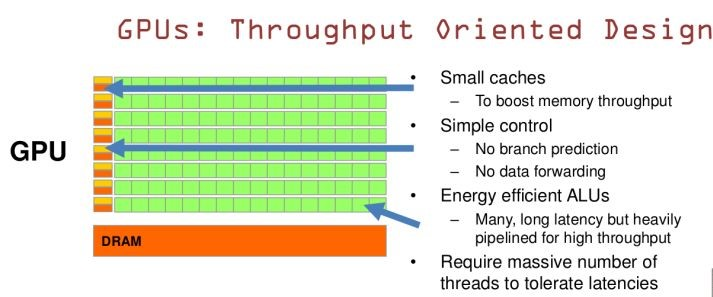
\includegraphics[scale=0.4]{figure/Gpu structure.jpg}
        \caption{GPU并行计算}
    \end{figure}

	与CPU擅长逻辑控制,串行的运算。和通用类型数据运算不同,GPU擅长的是大规模并发计算,如本算法中计算量大但简单的工作,因此可以设计GPU加速算法应用于本文的工作.
	
	\subsubsection{自动寻找种子算法设计}

	可以设计一个算法,自动寻找到三维图像中高亮像素点密集的区域,并生成一个三维的模型,通过选取模型的中间像素点,得到我们所需要的种子值。

	为了提高分割的精度,我们也可以通过对该点附近的多个点进行区域生长计算,取其中精度最高的点来作为我们得到的模型,注意到该算法实际上大大增加了时间上的消耗,但它为自动化区域增长分割算法提供了一种思路,此外,通过并行化GPU加速算法的设计与使用,也使得这种设想成为了一种可能。

	\subsection{总结和致谢}

    通过本学期的课程,我们学习到了很多关于图像处理的知识,而本次的大作业也是对我们所学知识的一次检测。在实现本次大作业的过程中,我们既感受到了图像处理的神奇,为所得到的结果而激动,同时也在查阅资料的过程中感受到了自己所学知识的不足,本学期所学的知识仅仅是冰山一角,图像需要我们进一步地深入学习,“路曼曼其修远兮,我将上下而求索。”
    
    最后,感谢老师和助教在本次大作业中给予我们的帮助的解答!

\end{document}
